%
% simplex.tex -- simplizes und Polyeder
%
% (c) 2021 Prof Dr Andreas Müller, OST Ostschweizer Fachhochschule
%
\section{Simplizes
\label{buch:section:simplexe}}
\rhead{Simplizes}
Die Idee, das Dreieck und seinen Rand zu unterscheiden verlangt,
dass wir zunächst Dreiecke und deren höherdimensionale Verallgemeinerungen,
die sogenannten Simplizes entwickeln müssen.

\subsection{Simplizes und Rand
\label{buch:subsection:simplices}}
Die Inzidenzmatrix eines Graphen hat einer Kante die beiden Endpunkte
mit verschiedenen Vorzeichen zugeordnet.

\subsubsection{Rand eines Dreiecks}
Dieses Idee soll jetzt verallgemeinert werden.
Der Rand des Dreiecks $\triangle P_0P_1P_2$ in
Abbildung~\ref{buch:homologie:figure:zusammenziehbar}
besteht aus den Kanten $P_0P_1$, $P_1P_2$ und $P_0P_2$.
Für eine algebraische Definition müssen die Kanten offenbar eine
Orientierung haben, die ist aber garantiert, da wir den Anfangs-
und Endpunkten einer Kante verschiedene Vorzeichen gegeben haben.
Dem Dreieck $\triangle$ werden dann die drei Kanten $k_{01}$, $k_{02}$
und $k_{12}$ zuogeordnet, aber mit zusätzlichen Vorzeichen, die
die Orientierung festhalten.
Durchläuft man den Rand von $\triangle$ in der Reihenfolge $P_0P_1P_2$,
dann muss die Kante $k_{02}$ ein negatives Vorzeichen erhalten.

Wir können diese Zuordnung wieder mit einer Matrix ausdrücken.
\[
\begin{matrix}
\text{$k_{01}$:}\mathstrut\\
\text{$k_{02}$:}\mathstrut\\
\text{$k_{12}$:}\mathstrut
\end{matrix}
\qquad
\partial
=
\begin{pmatrix*}[r]
1\mathstrut\\
-1\mathstrut\\
1\mathstrut
\end{pmatrix*}
\]

\subsubsection{Standardsimplizes}
Punkte, Kanten und Dreiecke sind die einfachsten Fälle sogenannter
Simplizes.
Wir formulieren die Definition dieser Objekte auf eine Weise,
die uns ermöglichen soll, sie auf beliebige Dimension zu verallgemeinern.

Die Strecke, die die Punkte $P$ und $Q$ miteinander verbindet,
kann beschrieben werden durch eine Parametrisierung
der Form
\begin{equation}
s_1
\colon
t
\mapsto
t\vec{p} + (1-t) \vec{q}
=
t_0 \vec{p} + t_1\vec{q},
\end{equation}
wobei die beiden positiven reellen Zahlen $t_0,t_1\in\mathbb{R}$ die
Bedingung $t_0 + t_1 = 1$ erfüllen.
Für ein eindimensionales Objekt brauchen wir also zwei Punkte und zwei
positive Parameter, die sich zu $1$ summieren.
Die Mengen $\triangle_1=\{ (t_0,t_1)\mid t_i\ge 0, t_0+t_1=1\}$ kann also
ganz allgemein als Parameterraum zur Beschreibung eines eindimensionalen Objektes
$\triangle_1$
mit den Endpunkten $0$ und $1$ dienen.
Eine Strecke ist also eine Abbildung der Form
\begin{equation}
s_1
\colon
\triangle_1 \to \mathbb{R}^N
:
(t_0,t_1)
\mapsto
t_0 \vec{p} + t_1\vec{q},
\end{equation}
und der Rand besteht aus den Punkten $s_1(0)$ und $s_1(1)$, wobei der
Anfangspunkt $s_1(0)$ mit einem negativen Vorzeichen versehen wird.

Für höhere Dimensionen brauchen wir auf analoge Weise erst wieder einen
geeigneten Parameterraum.
Die Menge
\begin{equation}
\triangle_n
=
\{(t_0,\dots,t_n)\in\mathbb{R}^{n+1}\mid t_i\ge 0,t_0+t_1+\dots+t_n=1\}
\subset\mathbb{R}^{n+1}
\label{buch:homologie:eqn:standardsimplex}
\end{equation}
beschreibt zum Beispiel für $n=2$ ein Dreieck und für $n=3$ ein 
Tetraeder.
\index{Tetraeder}%

\begin{definition}
Die Menge $\triangle_n$ von \eqref{buch:homologie:eqn:standardsimplex}
heisst das $n$-dimensionale Standardsimplex.
\index{Standardsimplex}%
\end{definition}

Die Standardbasisvektoren von  $\mathbb{R}^{n+1}$ werden mit $e_0,\dots,e_n$
bezeichnet und sind die Ecken des $n$-dimensionalen Standardsimplex.

\subsubsection{Simplizes in $\mathbb{R}^N$}
Gegeben $n+1$-Punkte $P_0,\dots,P_n$ mit Ortsvektoren
$\vec{p}_0,\dots,\vec{p}_n\in\mathbb{R}^N$, können wir eine Abbildung
\begin{equation}
s_n
\colon
\triangle_n
\to
\mathbb{R}^N
:
(t_0,\dots,t_n)
\mapsto
t_0\vec{p}_0
+
t_1\vec{p}_1
+
\dots
+
t_n\vec{p}_n
\end{equation}
Eine solche Abbildung verallgemeinert also den Begriff einer Strecke
in einem Raum $\mathbb{R}^N$  
auf höhere Dimensionen.
Sie ist durch die Eckpunkte vollständig vorgegeben, es reicht also
die Punkte $P_0,\dots,P_n\in\mathbb{R}^N$ zu kennen.

%\begin{definition}
%\label{buch:def:simplex}
%Ein $n$-dimensionales {\em Simplex} oder {\em $n$-Simplex} in $X$ ist eine
%stetige Abbildung $s_n\colon\triangle_n\to X$.
%\end{definition}
%
%Die Ecken des $n$-Simplex $\triangle_n$ sind die Standardbasisvektoren
%in $\mathbb{R}^{n+1}$.
%Mit $e_k$ bezeichnen wird die Ecke, deren Koordinaten $t_i=0$ sind für 
%$k\ne i$, ausser der Koordinaten $t_k$, die den Wert $t_k=1$ hat.


\begin{definition}
Ein $n$-Simplex in $\mathbb{R}^N$ ist die stückweise lineare Abbildung
$s\colon \triangle_n\to \mathbb{R}^N$ gegeben durch die Bilder der Eckpunkte
$P_i = s(e_i)$.
Wir schreiben auch $[P_0,P_1,\dots,P_n]$ für dieses Simplex.
\end{definition}

\subsubsection{Rechnen mit Simplizes}
Wir möchten später ein geometrisches Objekt aus Simplizes zusammensetzen.
Dies soll rein algebraisch geschehen, die einzelnen Simplizes sollen
formal als Basisvektoren eines abstrakten Vektorraums verwendet werden.
Damit das geht, müssen die Simplizes so platziert sein, dass
sie an den Rändern zusammenpassen.

Simplizes verschiedener Dimension in $\mathbb{R}^N$ können natürlich 
immer unterschieden werden, wir können also den Vektorraum in einzelne
Vektorräume aufteilen, einen für jede Dimension.
Der Vektorraum in Dimension $l$ wird von den $l$-dimensionalen Simplizes 
als Basis erzeugt und wir bezeichnen ihn mit $C_l$.
Da die Eckpunkte ein Simplex in $\mathbb{R}^N$ festlegen, ist ein
$l$-dimensionales Simplex, als ein Basisvektor von $C_l$ durch
das $l+1$-Tupel
\(
[P_0,\dots,P_l]
\)
von Punkten von $\mathbb{R}^N$ gegeben.
Der Vektorraum $C_l$ besteht dann aus Linearkombinationen
\[
C_l
=
\biggl\{
\sum x_{P_0\dots P_l} [P_0,\dots,P_l]
\;\bigg|\;
x_{P_0\dots P_l}\in\mathbb{R}
\biggr\}.
\]
Die Seitenflächen dieses Simplex sind die $l-1$-dimensionalen
Simplizes, die man erhält, indem man eine Ecke weglässt.
Wir bezeichnen mit $[P_0,\dots,\widehat{P_i},\dots,P_l] \in C_{l-1}$
Die Seitenfläche, die man durch Weglassen der Ecke $P_i$
erhalten hat.

\subsubsection{Rand eines Simplex}
Die Oberfläche eines Simplex ist nicht einfach die Summe der
Seitenflächen.
Die Kanten eines Dreiecks $[P_0,P_1,P_2]$ müssen so aneinandergefügt
werden, dass sie einen Weg um das Dreieck ergeben.
Beginnt man das Dreieck in Richtung der Kanten
$[P_0,P_1]$ und $[P_1,P_2]$ zu umlaufen, trifft man in
``verkehrter'' Richtung auf die Kante $[P_0,P_2]$.
Für den Rand des Dreiecks muss man also diese Kante mit negativem
Vorzeichen zählen:
\begin{align*}
\partial_3 \colon
[P_0,P_1,P_2]
\mapsto
[P_0,P_1]
+ [P_1,P_2]
- [P_0,P_2]
&=
[\widehat{P_0},P_1,P_2]
-[P_0,\widehat{P_1},P_2]
+[P_0,P_1,\widehat{P_2}]
\\
&=
\sum_{i=0}^l (-1)^i [P_0,\dots,\widehat{P_i},\dots,P_3]
\end{align*}
Dies ist auch die Art, wie Kanten des Dreiecks $\triangle$ 
in Abbildung~\ref{buch:homologie:figure:zusammenziehbar}
orientiert wurden.

\begin{definition}
\label{buch:def:randoperator}
Der Randoperator ordnet einem $l$-Simplex dessen $l-1$-dimensonale
Seitenflächen mit alternierenden Vorzeichen zu:
\[
\partial_l : [P_0,\dots,P_l]
\mapsto
\sum_{i=0}^l (-1)^i [P_0,\dots,\widehat{P_i},\dots,P_l].
\]
\end{definition}

\subsubsection{Inzidenzmatrix eines gerichteten Graphen und Randoperator}
In Abschnitt~\ref{buch:graphen:subsection:inzidenzmatrix} wurde die
Inzidenzmatrix eines gerichteten Graphen $G=(V,E)$ definiert.
Seien $V=\{v_1,\dots,v_n\}$ die Vertizes des Graphen und
$E=\{e_1,\dots,e_m\}$ die Kanten. 
Gibt es eine Kante $e_k = (v_i,v_j)\in E$ im Graphen, dann hat die Inzidenzmatrix
in Spalte $k$ die Einträge $-1$ in Zeile $i$ und $+1$ in Zeile $j$.
Die Kante $e_k$ können wir als eindimensionales Simplex $[v_i,v_j]$
betrachten.
Die Adjazenzmatrix ordnet ihm die Linearkombination
\[
A(G)\colon e_k=[v_i,v_j] \mapsto -[v_i] +[v_j]
= (-1)^0 [\widehat{v_i},v_j] + (-1)^1 [v_i,\widehat{v_j}]
=
\partial_2 [v_i,v_j]
\]
zu.
Die Adjazenzmatrix eines Graphen kann man also als den Randoperator
$\partial_1$ betrachten, der auf den als $1$-dimensionale Simplizes
betrachteten Kanten des Graphen wirkt.

\subsubsection{Der Rand des Randes}
Der Rand eines Tetraeders setzt sich aus vier Dreiecken
zusammen.
Jede Kante gehört zu genau zwei Seitenflächen. 
Wenn die Dreiecke alle so orientiert sind, dass sie ``von ausserhalb''
des Tetraeders betrachtet positiv orientiert sind, dann wird jede
Kante zweimal in jeder Richtung durchlaufen.
Bildet man den Rand all dieser Seitenflächen, kommte jede Kante
einmal mit positivem und einmal mit negativem Vorzeichen vor,
die Summe ist $0$.

Ganz allgemein gilt, dass der Rand des Randes verschwindet.

\begin{satz}
\label{buch:homologie:satz:randrand}
Es gilt $\partial_{l-1}\circ\partial_l=0$.
\end{satz}

\begin{proof}[Beweis]
Der Rand des Simplex $[P_0,\dots,P_l]$ ist
\[
\partial_l[P_0,\dots,P_l]
=
\sum_{i=0}^l (-1)^i [P_0,\dots,\widehat{P_i},\dots,P_l].
\]
Darauf muss jetzt der Randoperator $\partial_{l-1}$ angewendet
werden.
Dabei wird auf der rechten Seit jeweils der Index $i$ des weggelassenen
Punktes übersprungen, bei der Bildung der
Summe müssen die Teile vor und nach $i$ daher separat betrachtet werden:
\begin{align}
\partial_{l-1}\partial_l[P_0,\dots,P_l]
&=
\sum_{i=0}^l (-1)^i \partial_{l-1}[P_0,\dots,\widehat{P_i},\dots,P_l]
\notag
\\
&=
\sum_{i=0}^l (-1)^i
\biggl(
\sum_{j<i} (-1)^j
[P_0,\dots,\widehat{P_j},\dots,\widehat{P_i}\dots,P_l]
\notag
\\
&\hspace*{2cm}
+
\sum_{j>i} (-1)^{j-1}
[P_0,\dots,\widehat{P_i},\dots,\widehat{P_j}\dots,P_l]
\biggr)
\label{buch:homologie:eqn:randrand}
\\
&=
\sum_{j<i} (-1)^{i+j}
[P_0,\dots,\widehat{P_j},\dots,\widehat{P_i}\dots,P_l]
-
\sum_{j>i} (-1)^{i+j}
[P_0,\dots,\widehat{P_i},\dots,\widehat{P_j}\dots,P_l]
\notag
\end{align}
Auf der letzten Zeile sind die Summen über alle Paare
$(i,j)\in\{0,\dots,n\}^2$ zu erstrecken, die die zusätzliche
Bedingung $j<i$ bzw.~$j>i$ erfüllen.
Der Exponent $j-1$ im zweiten Term von
\eqref{buch:homologie:eqn:randrand}
trägt der Tatsache Rechnung,
dass der Index $i$ übersprungen worden ist.
In der zweiten Summe kann man die Summationsindizes umbenennen,
also $i$ durch $j$ ersetzen und umgekehrt, dann entsteht
\begin{align*}
\partial_{l-1}\partial_l[P_0,\dots,P_l]
&=
\sum_{j<i} (-1)^{i+j}
[P_0,\dots,\widehat{P_j},\dots,\widehat{P_i}\dots,P_l]
\\
&\qquad
-
\sum_{i>j} (-1)^{j+i}
[P_0,\dots,\widehat{P_j},\dots,\widehat{P_i}\dots,P_l]
\\
&=0.
\qedhere
\end{align*}
\end{proof}

\subsection{Polyeder}
\begin{figure}
\centering
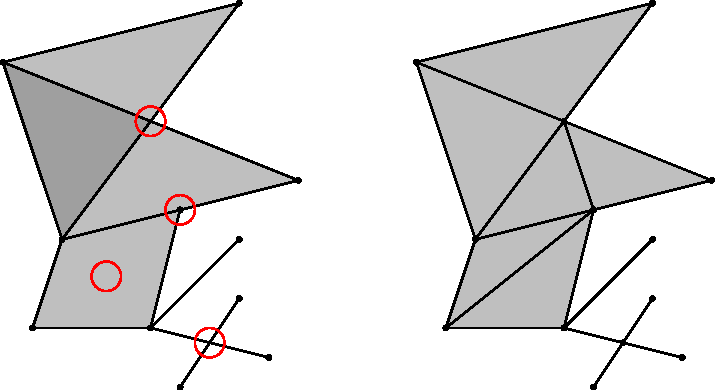
\includegraphics{chapters/95-homologie/images/polyeder.pdf}
\caption{Aufbau eines zweidimensionalen Polyeders aus
verschiedenen Simplizes.
Die Schnittmenge zweier Simplizes muss ein Untersimplex beider Simplizes
sein.
Die roten Kreise im linken Bild weisen auf verschiedene Situationen
hin, wo das diese Bedingung nicht erfüllt ist.
In rechten Bild sind zusätzliche Simlizes hinzugefügt worden, um
die Bedingungen eines Polyeders zu erfüllen.
\label{buch:homologie:figure:polyeder}}
\end{figure}
Aus einzelnen Simplizes können jetzt kompliziertere geometrische
Objekte gebaut werden.
Ein Graph ist ein Beispiel für ein geometrisches Objekt, welches
als Vereinigung von 1-Simplizes entsteht.
Die Vereinigung ist aber nicht beliebig, vielmehr ist die Schnittmenge
zweier beliebiger 1-Simplizes immer entweder leer, eine Menge 
mit nur einem Vertex oder ein ganzes 1-Simplex.

Für höhere Dimensionen muss diese Idee ausgedehnt werden auf
höherdimensionale Simplizes.
In einem Graphen dürfen sich Kanten nicht in einem inneren Punkt treffen,
sondern nur in Endpunkten.
Verallgemeinert auf höherdimensionale Simplizes kann man dies als die
Bedingung formulieren, dass die Schnittmenge zweier beliebiger
Simplizes immer Untersimplizes beider Simplizes sein müssen.
Wir fassen dies zusammen in der folgenden Definition.

\begin{definition}
\index{Polyeder}%
\index{Dimension eines Polyeders}%
\index{Polyeder, Dimension eines}%
Ein {\em Polyeder} ist eine Vereingung von endlich vielen Simplizes derart,
dass die Schnittmenge zweier beliebiger Simplizes immer ein Untersimplex
beider Simplizes ist.
Die {\em Dimension} des Polyeders ist die grösste Dimension der darin
enthaltenen Simplizes.
\end{definition}

Ein Graph ist nach dieser Definition ein eindimensionales Polyeder.
Die Mengen in der Abbildung~\ref{buch:homologie:figure:polyeder}
ist kein Polyeder, kann aber leicht zu einem Polyeder gemacht werden,
indem man einzelne Kanten mit zusätzlichen Punkten unterteilt.
Auch müssen die zweidimensionalen Simplizes aufgeteilt werden.

Abbildung~\ref{buch:homologie:figure:polyeder} zeigt auch, dass
die Darstellung einer Punktmenge als Polyeder nicht eindeutig ist.
Man kann die Kanten und Flächen jederzeit weiter unterteilen, ohne
dass sich die Gestalt der gesamten Menge dadurch ändert.

\subsection{Triangulation
\label{buch:subsection:triangulation}}
Unser Ziel ist, geometrische Objekte besser verstehen zu können.
Dabei sind uns Deformationen und sogar Knicke egal, es interessiert uns
nur die ``Gestalt'' oder ``Topologie'' des Objekts.
Entfernungen zwischen Punkten sind ebenfalls von untergeordneter 
Bedeutung, da sie bei Deformation nicht erhalten bleiben.
Der Begriff des ``topologischen Raumes'' fasst diese Ideen mathematisch
präzise ein, eine genaue Definition würde aber an dieser Stelle zu weit
führen.
Stattdessen beschränken wir uns auf eine Klasse von Punktmengen, die man
mit Simplizes beschreiben kann.

Ein topologischer Raum zeichnet sich durch einen Nachbarschaftsbegriff
von Punkte aus, der erlaubt zu definieren, was eine stetige Abbildung ist.
Ein stetige Abbildungen bildet nahe beeinander liegende Punkte wieder
auf nahe beeinander liegende Punkte ab.
Dass nahe liegende Punkte nicht plötzlich auf weit auseinander liegende
Punkte abgebildet werden gibt die Intuition wieder, dass Deformationen
möglich sein sollen, dass der Raum dabei aber nicht ``reissen'' darf.
Zwei topologische Räume $X$ und $Y$ können daher als ``gleichgestaltig''
betrachtet werden, wenn es zwei stetige Abbildungen $f\colon X\to Y$
und $g\colon Y\to X$ gibt, die zu einander invers sein.
Oder wenn sich $X$ stetig auf $Y$ abbilden lässt, so dass auch die
Umkehrabbildung stetig ist.
Eine solche Abbildung heisst ein {\em Homöomorphismus}, die beiden Räume
$X$ und $Y$ heissen {\em homöomorph}.

Eine Kugel ist natürlich kein Polyeder, aber sie kann leicht homöomorph
auf ein dreidimensionales Simplex abgebildet werden.

\begin{beispiel}
\label{buch:homologie:projektion}
Sei $T$ ein reguläres Tetraeder mit den Ecken auf der dreidimensionalen
Einheitskugel $B^3$.
Für jeden Richtungsvektor $x\ne 0$ sei $l(x)$ Entfernung vom Mittelpunkt des
Tetraeders bis zum Durchstosspunkt einer Geraden durch den Mittelpunkt
mit Richtungsvektor $x$ durch die Oberfläche des Tetraeders.
Dann sind die Abbildungen
\[
f\colon
T\to B^3
:
x \mapsto\begin{cases}
\displaystyle
\frac{x}{l(x)}&\quad\text{für $x\ne 0$}\\
0&\quad\text{für $x=0$}
\end{cases}
\qquad\text{und}\qquad
g\colon
B^3\to T
:
x \mapsto\begin{cases}
l(x) x&\quad\text{für $x\ne 0$}\\
0&\quad\text{für $x=0$}
\end{cases}
\]
zueinander inverse stetige Abbildungen oder Homöomorphismen.
Dies funktioniert natürlich nicht nur ein Tetraeder, sondern für jedes
beliebige konvexe Polyeder.
\end{beispiel}

Im Folgenden sollen daher nur solche topologischen Räume untersucht werden,
die homöomorph sind zu einem Polyeder.
Man nennt die homöomorphe Abbildung eines Polyeders auf so einen Raum
auch eine Triangulation.
Triangulationen reduzieren die algebraischen Untersuchungen auf jene
von Polyedern.
Durch Unterteilung der Simplizes in kleiner Simplizes kann eine solche
Triangulation beliebig verfeinert werden.






